\section{Observations and Analysis}\label{sec:analysis}
% Owner: P1. Budget 1.90 page incl. Fig. 1 and Table I. Plan: ../OUTLINE_V2.md section III.
% Pointer convention: every line with a number or a literature claim ends in a % comment.
% EV = docs/term-paper/evidence/README.md; CM = evidence/COST_MODEL.md; EM = EVIDENCE_MAP.md row; OB = contracts/src/OrderBook.sol.

Each market is one \texttt{OrderBook} contract that holds every order's tokens in escrow until it fills or is cancelled~\cite{repo8753521}. % OB:214-221 (_pullEscrow)
Orders are ranked by price and then by an internal sequence number stamped when they enter the book, and every fill executes at the price of the resting order, the \emph{maker}, rather than the incoming order, the \emph{taker}. % OB:38-40, 115, 276
Three constants bound the work of one call: a taker makes at most ten fills (\texttt{MAX\_MATCHES\_PER\_TX}), an insertion walks past at most 100 better-ranked orders (\texttt{MAX\_INSERT\_SCAN}), and amounts are multiples of $10^{9}$ base units, so the smallest order (one \emph{lot}) is $10^{-9}$ of a token (\texttt{LOT\_SIZE}). % OB:18-21; EM C1a, C4a
A taker that runs out of fills rests in the book with its remainder, and anyone may later call \texttt{matchOrders} to clear a crossed book or \texttt{triggerStopOrders} to activate stop orders, without any reward. % OB:67-68, 103-119, 127-145; EM C6a
A stop-limit order becomes eligible when \texttt{lastTradePrice}, which every fill of any size overwrites, reaches its trigger. % OB:242-248, 291; EM C2a

We assume an adversary, Mallory, who sees pending transactions and the whole public book, can place and cancel orders from several accounts, can call the two keeper functions, and can deploy a contract that makes several calls in one transaction. % EM C1b caveat, C3d
She cannot move other users' escrow, forge their orders, or control consensus; any ordering advantage she has comes from landing before or after a victim, which Daian et al. observed being bought with transaction fees on proof-of-work Ethereum~\cite{src01daian2020}. % [01] p. 1, p. 5 to 6 Sec. III-C (PGAs, F1); EM C1e
Bob and Carol are honest traders; every experiment is a deterministic Foundry test on a local chain. % EV header (forge 1.8.6)

\subsection{C1: Fill-Cap Sandwich}\label{sec:c1}
\emph{Component and cause.}
The ten-fill cap in \texttt{placeLimitOrder} lets Mallory spend a victim's fills on dust: once the cap is reached, the unfilled remainder is inserted as a resting order at the victim's own limit, even if it still crosses a better order on the other side. % OB:20, 67-68; EM C1a
Fig.~\ref{fig:sandwich} traces the case recorded in our audit as issue 007. % OrderBook.Regression.t.sol:184
Bob rests an ask for 10 base at 1.5. % EV E1 setup (TermPaper.t.sol:97)
Mallory places ten one-lot asks at 1.499 just before Carol's buy of 10 at a limit of 2.0. % EV E1 setup
Carol's ten fills buy only $10^{-8}$ base, so almost all of her order rests as a bid at 2.0 above Bob's ask. % EV E1 setup; OB:67-68
Mallory then sells into Carol's bid, where Carol is now the maker and the price is 2.0, and buys Bob's ask at 1.5. % OB:276 (maker price)

% Fig. 1: C1 fill-cap sandwich (issue 007), three lifelines, four steps. Needs \usepackage{tikz}.
% Prices and sizes: evidence/README.md E1 setup (TermPaper.t.sol:97); engine lines OrderBook.sol:20, 67-68, 115.
% Keeper window: E9, test_E9_keeperClearsBeforeBackrun_sandwich.
\begin{figure}[t]
\centering
\resizebox{\columnwidth}{!}{%
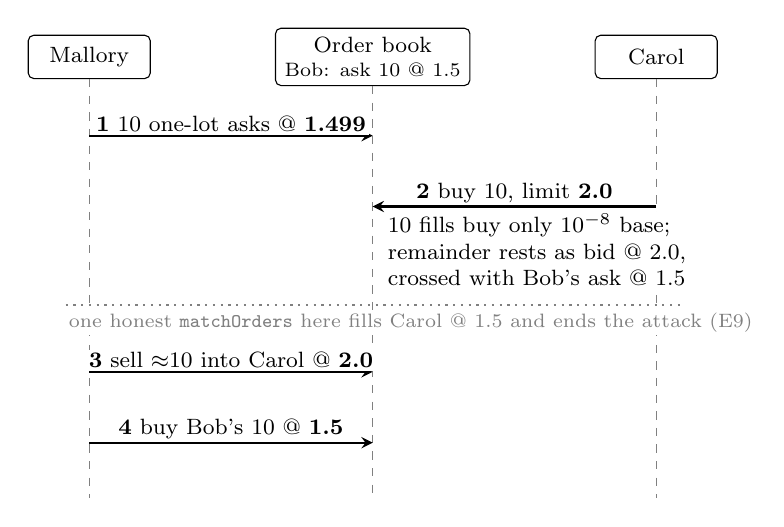
\begin{tikzpicture}[
  font=\footnotesize,
  >=stealth,
  life/.style={draw, rounded corners=2pt, minimum width=1.55cm, minimum height=0.55cm, align=center},
  msg/.style={->, thick},
  lbl/.style={fill=white, inner sep=1pt, align=center}
]
% Lifeline heads. x: Mallory 0, book 3.6, Carol 7.2 (scaled to the column below).
\node[life] (M) at (0,0) {Mallory};
\node[life] (B) at (3.6,0) {Order book\\[-1pt]\scriptsize Bob: ask 10 @ 1.5};
\node[life] (C) at (7.2,0) {Carol};
\draw[dashed, gray] (M.south) -- (0,-5.6);
\draw[dashed, gray] (B.south) -- (3.6,-5.6);
\draw[dashed, gray] (C.south) -- (7.2,-5.6);

% Step 1: dust front-run.
\draw[msg] (0,-1.0) -- node[lbl, above] {\textbf{1} 10 one-lot asks @ \textbf{1.499}} (3.6,-1.0);
% Step 2: victim order uses its 10 fills on dust; remainder rests at its limit.
\draw[msg] (7.2,-1.9) -- node[lbl, above] {\textbf{2} buy 10, limit \textbf{2.0}} (3.6,-1.9);
\node[lbl, align=left, anchor=west] at (3.75,-2.45)
  {10 fills buy only $10^{-8}$ base;\\remainder rests as bid @ 2.0,\\crossed with Bob's ask @ 1.5}; % EV E1 setup; OB:67-68
% Keeper window between steps 2 and 3 (E9).
\draw[gray, thick, dotted] (-0.3,-3.15) -- (7.5,-3.15);
\node[lbl, text=gray, anchor=west] at (-0.3,-3.38)
  {\scriptsize one honest \texttt{matchOrders} here fills Carol @ 1.5 and ends the attack (E9)};
% Step 3: back-run, Carol is now the maker so the price is her limit.
\draw[msg] (0,-4.0) -- node[lbl, above] {\textbf{3} sell $\approx$10 into Carol @ \textbf{2.0}} (3.6,-4.0);
% Step 4: buy Bob's cheaper ask.
\draw[msg] (0,-4.9) -- node[lbl, above] {\textbf{4} buy Bob's 10 @ \textbf{1.5}} (3.6,-4.9);
\end{tikzpicture}}
\caption{C1 fill-cap sandwich (issue 007). Carol pays 19.99999999499 quote for 10 base instead of 15.0;
Mallory gains the 4.99999999499 difference before gas (E1). Step 3 must land before any \texttt{matchOrders} call.} % EV E1 33% row; EV E9
\label{fig:sandwich}
\end{figure}
% Caption numbers: evidence/README.md E1, 33% row (Carol quote paid 19.999999994990, Mallory profit 4.999999994990).


\emph{Impact.}
Carol receives her 10 base but pays 19.99999999499 quote instead of 15.0, and Mallory's quote profit equals that overpayment exactly. % EV E1, 33% row; asserted TermPaper.t.sol:146-148
Carol never pays above her own limit and no escrow is lost, so every accounting check passes; the loss is the gap between her limit and the best price that was resting in the book. % EM C1b; OrderBook.Regression.t.sol:184
The loss is linear in the victim's limit slack: 0.015, 0.15, 0.75 and 5.0 quote at 0.1\%, 1\%, 5\% and 33\% above the ask, while Mallory's cost stays at 3{,}910{,}616 gas over 12 transactions (Table~\ref{tab:experiments}). % EV E1 rows; CM table
These are profits before gas. % CM header
With $Q$ the dollar value of one quote token and $P$ the dollar price of ETH, the attack pays only while the gas price in gwei stays below $K Q / P$, where $K$ is $3.84$ at 0.1\% slack and $1278.57$ at 33\%. % CM formula and table (E1 rows)
Gas is fixed by the number of transactions while profit grows with order size and slack, so large orders with loose limits are the targets. % CM reading notes

\emph{Ordering dependence.}
The attack needs Mallory's back-run to land before anyone calls \texttt{matchOrders}. % EV E9 "Proves"
In \texttt{matchOrders} the order that entered the book first is the maker, so one honest call of 153{,}587 gas fills Carol against Bob at 1.5 and leaves Mallory $10^{-11}$ quote worse off, marked at 1.5 (Table~\ref{tab:experiments}). % OB:115; EV E9 row 1

\emph{Comparable published cases.}
In the front-running taxonomy of Eskandari et al., C1 is an insertion attack: the attacker needs the victim's transaction to run and trades against it at the victim's price, and fully on-chain order books are named as generally open to insertion and displacement~\cite{src02eskandari2019}. % [02] p. 4 to 5 Sec. 3 (F1, F2), p. 7 Sec. 4.1 (F3); EM C1c
Daian et al. show a bot capturing a crossed order book on an order-book DEX after a priority gas auction~\cite{src01daian2020}. % [01] p. 4 to 6 Sec. III-B/C (TokenStore, F3); EM C1f
The closest measured case is the sandwich attack on automated market makers (AMMs), with 750{,}529 attacks found on Ethereum~\cite{src05qin2022}. % [05] p. 4 Sec. IV-A2 (F2); EM C1d
That mechanism is only analogous: an AMM sandwich moves a pool price, while C1 moves a victim into the maker role. % EM C1d caveat; notes/PHASE4_GAPS.md gap a

% Table I (max 9 rows). Numbers from docs/term-paper/evidence/README.md, confirmed identical in
% evidence/rerun-2026-11-25.txt (forge 1.8.6). Gas = attacker gas over all its transactions, local Foundry
% measurement. E2 and E8 "gain" is a paper gain marked at the last honest price 2.0. Profits are before gas.
% Dropped rows (in text only): E1 0.1% (0.015) and 5% (0.75); E2 depth 5 (3.0 / 2.5); E9 snipe, keeper first (0).
\begin{table}[t]
\caption{Attack results in quote tokens, victim order 10 base. Gains are before gas; E2 and E8 gains are paper gains marked at 2.0. Loss is the victim's, gain and gas (transactions) the attacker's; gas measured locally with Foundry 1.8.6. E8 runs on the research copy with M1}
\label{tab:experiments}
\centering
\footnotesize
\setlength{\tabcolsep}{4pt}
\begin{tabular}{@{}llrrr@{}}
\toprule
Exp. & Case & Loss & Gain & Gas (tx) \\
\midrule
E1 & Sandwich, 1\% slack & 0.15 & 0.15 & 3{,}910{,}616 (12) \\ % evidence/README.md E1, 1% row: 0.14999999984
E1 & Sandwich, 33\% (issue 007) & 5.0 & 5.0 & 3{,}910{,}616 (12) \\ % E1, 33% row: 4.99999999499
E9 & Sandwich, keeper first & 0 & 0 & 3{,}222{,}611 (10) \\ % E9 table, row 1 (net -1e-11 at 1.5)
E2 & Stop hunt, depth 0 & 5.0 & 5.0 & 1{,}158{,}241 (4) \\ % E2 table, depth 0
E2 & Stop hunt, depth 10 & 1.0 & 0 & 1{,}173{,}905 (4) \\ % E2 table, depth 10
E8 & Stop hunt, minOrder 0.1 & 5.0 & 5.0 & 1{,}160{,}501 (4) \\ % E8 table
E3 & Stop snipe & 10.0 & 10.0 & 4{,}942{,}713 (13) \\ % E3 table: received 10.000000011 vs 20.0; profit 9.999999989
E9 & Stop snipe, one tx & 10.0 & 10.0 & 3{,}588{,}665 (1) \\ % E9 table, row 3
E4 & Dust wall, bids blocked & \multicolumn{2}{r}{11 tx to clear} & 67{,}436{,}118 (101) \\ % E4 table; defender 8,056,221 gas
\bottomrule
\end{tabular}
\end{table}


\subsection{C2 and C3: Stop-Order Manipulation}\label{sec:c23}
\emph{C2, stop hunt.}
Because any fill sets \texttt{lastTradePrice} and the engine does not stop a trader filling their own order, Mallory can move the reference price with a one-lot trade against herself. % OB:251-268 (no trader check), 291; EM C2a, C2b
In our test the last honest trade is at 2.0 and Carol has a sell stop with trigger 1.95 and limit 1.5; one self-trade of one lot at 1.95 fires her stop. % EV E2 setup; asserted TermPaper.t.sol:179-180
Measured against 2.0, Carol's shortfall is 5.0, 3.0 and 1.0 quote as the honest bid depth at 1.90 grows from 0 to 5 to 10 base. % EV E2 table; EM C2c
Mallory's 5.0 gain at zero depth is a paper gain marked at 2.0, and part of the shortfall is ordinary stop slippage. % EV E2 per-test review (1), (3)
A minimum order size does not change this: with a minimum of 0.1 base the self-trade is simply 0.1 base, it still nets to zero for Mallory, and the shortfall is still 5.0 (E8). % EV E8 table; EM M1b
Self-trades occur on real order-book DEXs that match off-chain, with 58{,}791 on EtherDelta alone~\cite{src12victor2021}, and in foreign exchange data from 1996 to 2000 stop orders cluster near round numbers and amplify price moves once triggered~\cite{src13osler2005}. % [12] p. 7 Sec. 6.1 (F4); [13] p. 7 Sec. I-A, p. 1 (F1, F3); EM C2d, C2f
Osler reports deliberate stop running only as market lore, and her stops were private, while ours are public. % [13] p. 3 (F7), p. 9 (F8)
We did not find a study of stop hunting through reference-price manipulation in crypto markets. % notes/PHASE4_GAPS.md gap b

\emph{C3, stop snipe.}
\texttt{triggerStopOrders} gives the whole call one budget of ten fills, so an activated stop that finds dust first can run out of fills and rest at its own limit. % OB:131, 141-142; EM C3a
In E3, with Bob bidding 10 at 2.0 and Carol holding a sell stop with trigger 2.0 and limit 1.0, Mallory places ten one-lot bids at 2.1, calls the trigger, buys Carol's crossed remainder at 1.0 and sells it to Bob at 2.0. % EV E3 setup
Carol receives 10.000000011 quote instead of 20.0, and Mallory keeps 9.999999989. % EV E3 table; EM C3b
The stop still executes within the limit Carol chose; the loss is against Bob's resting bid. % EM C3b
An honest \texttt{matchOrders} between the trigger and the back-run defeats this version, as in C1, but Mallory can place the dust, call the trigger and back-run inside one contract call: the same 9.999999989 profit for 3{,}588{,}665 gas in one transaction (E9). % EV E9 rows 2 and 3; EM C3d

C3 is the stronger finding for three reasons. % EM C3d
First, the one-transaction form leaves no gap in which a keeper can act, so it needs no ordering control around Carol's transaction; the only race is to be the first to call the trigger once the stop is eligible. % EV E9 "Proves"
Second, it takes about half of the victim's proceeds, against a third of the honest cost in C1. % EV E3 (10 of 20); EV E1 33% row (5 of 15)
Third, we argue it hits the order meant to protect the victim: a stop-loss limit is set wide so that it executes in a fall, and that width is what Mallory takes. % EV E3 setup (limit 1.0 vs trigger 2.0)
Babel et al. describe the same pattern of ordering around a price source to trigger liquidations and payouts~\cite{src08babel2023}, although not for stop orders. % [08] p. 18 Sec. 4.2 (F7); EM C3c

\subsection{C4: Dust Wall, a Security versus Scalability Trade-off}\label{sec:c4}
The insertion cap that keeps placement gas bounded also lets 101 resting orders block the side of the book behind them, because a new order that would walk past more than 100 better-ranked orders reverts with \texttt{BookTooDeep}. % OB:21, 313-314, 327-328; EM C4a
In E4 Mallory places 101 one-lot bids just below the best ask, after which every new non-crossing bid reverts, including one far below at 1.0. % EV E4 table; asserted TermPaper.t.sol:278-282
Clearing the wall took a defender 11 transactions and 8{,}056{,}221 gas, while building it cost Mallory 67{,}436{,}118 gas and locked only $1.5\times10^{-7}$ quote. % EV E4 table; asserted TermPaper.t.sol:298; CM griefing table
The attack is cheap in capital but costs 8.4 times the defender's gas, in line with the observation that growing a data structure costs about ten times more gas than iterating it~\cite{src15grech2018}. % CM griefing table; [15] p. 23 Sec. 6.4 (F10); EM C4b, C4d
We argue that gas is therefore the only barrier, and a weak one where gas is cheap: for an on-chain call market on an Arbitrum testnet, Moosavi and Clark report a 99.88\% cut in layer-one gas, not counting the layer-two work~\cite{src09moosavi2023}. % [09] p. 7 Table 6 (F6); EM S3 (Rinkeby, excludes L2 work)
We did not measure the wall on a layer two. % OPEN_QUESTIONS (none run)
Before issue 006 was fixed the same dust blocked every stop activation; now an activated stop that cannot enter the book is cancelled and refunded, so dust can still cancel another user's stop. % docs/ai-audit/issues/006; OrderBook.Stop.t.sol:620; OB:142; EM C4c

\subsection{C5 and C6: Tokens and Keepers}\label{sec:c56}
These two are reasoning from the code without an experiment. % OPEN_QUESTIONS weak C5b, C6b
\emph{C5.} Anyone can create a market for any 18-decimal token, and each fill pushes tokens to both traders inside settlement, so a token that refuses transfers to a chosen address would make every fill against that address revert. % MarketFactory.sol:27; OB:49, 296-298; EM C5a, C5b
This is the push-payment denial of service known from Ethereum contracts~\cite{src15grech2018}; no test reproduces it here. % [15] p. 7 to 8 Sec. 3.2 (F5); EM C5d
\emph{C6.} \texttt{matchOrders} and \texttt{triggerStopOrders} pay their callers nothing, yet C1 and C3 are both decided by who calls first. % OB:103-119, 127-145; EM C6a
Who pays to close an on-chain market is an open design problem in prior work~\cite{src09moosavi2023}, and we have no data on how long a crossed book or an eligible stop would wait on a public chain. % [09] p. 11 to 12 Sec. 6.3 (F9); EM C6b caveat
